% LTeX: enabled=false
\documentclass[a4paper,11pt,oneside]{article}

\usepackage{placeins}

\makeatletter
\AtBeginDocument{%
  % Modifying section command to include FloatBarrier
  \expandafter\renewcommand\expandafter\section\expandafter
    {\expandafter\@fb@secFB\section}%
  % Modifying subsection command to include FloatBarrier
  \expandafter\renewcommand\expandafter\subsection\expandafter
    {\expandafter\@fb@secFB\subsection}%
  
  \newcommand\@fb@secFB{\FloatBarrier
    \gdef\@fb@afterHHook{\@fb@topbarrier \gdef\@fb@afterHHook{}}}%
  
  \g@addto@macro\@afterheading{\@fb@afterHHook}%
  \gdef\@fb@afterHHook{}%
}
\makeatother

\usepackage[english]{babel}

\usepackage[T1]{fontenc}

\usepackage[utf8]{inputenc}

\usepackage{graphicx}
\usepackage{cite}
\usepackage{url}
\usepackage{ifthen}
\usepackage{listings}
\usepackage{xcolor}
\usepackage{blindtext} % https://tex.stackexchange.com/questions/111948/what-is-a-overfull-hbox-9-89561pt-too-wide

\usepackage{helvet} % Add sans-serif font package
\renewcommand{\familydefault}{\sfdefault} % Set sans-serif as default

\graphicspath{{images/}}

\usepackage[]{hyperref}
\usepackage{url}



\def \lstlistingname {SQL}
\lstset{
  language=SQL,
  tabsize=2,
  numbers=left,
  frame=L,
  floatplacement=hbtp,
  basicstyle=\ttfamily\small,
  keywordstyle=\color{blue},
  stringstyle=\color{red},
  commentstyle=\color{green},
  captionpos=b, % This sets the caption below the listing
  showstringspaces=false
}

% LTeX: enabled=true

\title{Database Methodology - SQLite Implementation Tools}

% Write the name and user namn for all contributors, se below for \and
\author{Edwin Sundberg \url{edwin.sundberg@dsv.su.se}}
% \and Person 2 \url{username2}

\begin{document}

\maketitle \pagebreak

% https://tex.stackexchange.com/questions/111948/what-is-a-overfull-hbox-9-89561pt-too-wide
\begin{sloppypar}  

\tableofcontents \pagebreak

% No one to thank yet
% \section{Acknowledgements}
% \label{acknowledgements}
% Thank you to the following people for reporting issues and contributing to this document:
% \begin{itemize}
%     \item Person 1 \url{username1}
%     \item Person 2 \url{username2}
%     \item Person 3 \url{username3}
% \end{itemize}

% TODO: Don't write "we", "I" or "us".

% TODO: Consistently use DBeaver Community or DBeaver, not both. (prob should be done with definition)

\section{The Database Model}
\label{exampleDatabaseModel}
In this document we will be using a simple database model which represents an email system, where users are able to create multiple recipient addresses and receive all incoming emails to one or more inboxes. All inboxes can be shared with other users in the system and receiving email may optionally be encrypted with a provided public key (see \url{https://en.wikipedia.org/wiki/Public-key_cryptography}). 
% TODO: Use cite for url instead

The original domain correct UML class diagram can be seen in figure \autoref{fig:originalUMLClassDiagram}. And the corresponding database model can be seen in figure \autoref{fig:originalDatabaseModel}. This document will not go into details on how or why the database model is created this way but rather focus on how to use the SQLite Modelling Tools to implement the database model. For details on how to go to a RDBMS friendly model from a domain model see lecture slides and literature.

% model/{database_friendly, instance, original_uml_class_diagram}.png
\begin{figure}[htb]
    \centering
    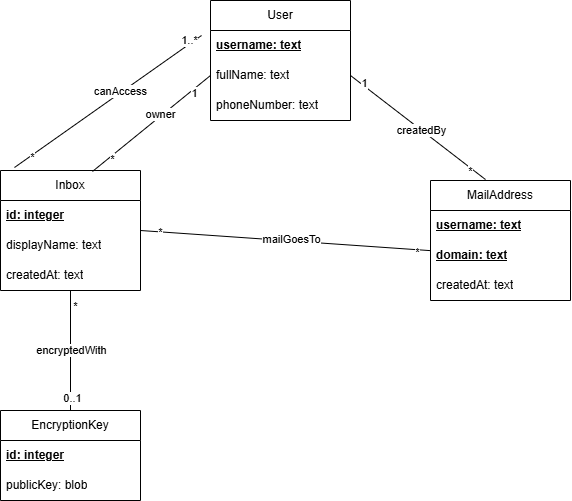
\includegraphics[width=1\textwidth]{model/original_uml_class_diagram.png}
    \caption{The original UML class diagram for the email system.}
    \label{fig:originalUMLClassDiagram}
\end{figure}

\begin{figure}[htb]
    \centering
    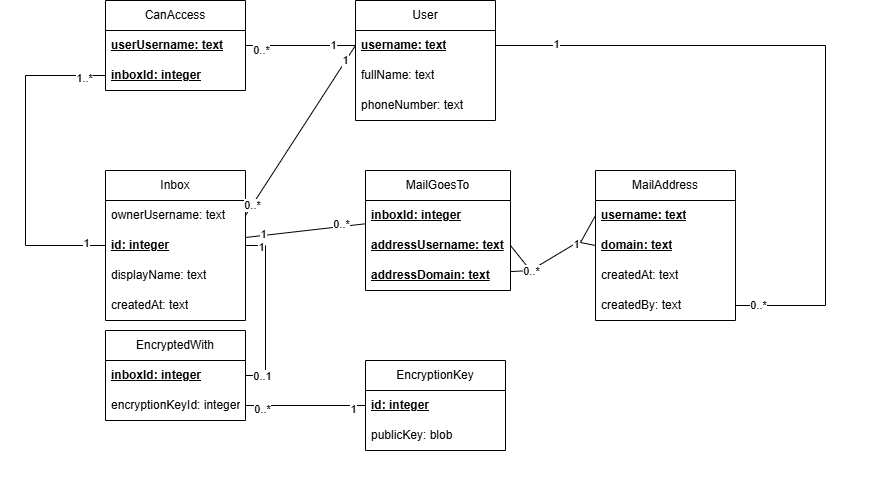
\includegraphics[width=1\textwidth]{model/database_friendly.png}
    \caption{The database model for the email system.}
    \label{fig:originalDatabaseModel}
\end{figure}

To further exemplify the database model we will also provide an instance of the database model in figure \autoref{fig:instanceDatabaseModel}. This instance will be used in the examples below to show how to insert data using the SQLite Implementation Tools.

\begin{figure}[htb]
    \centering
    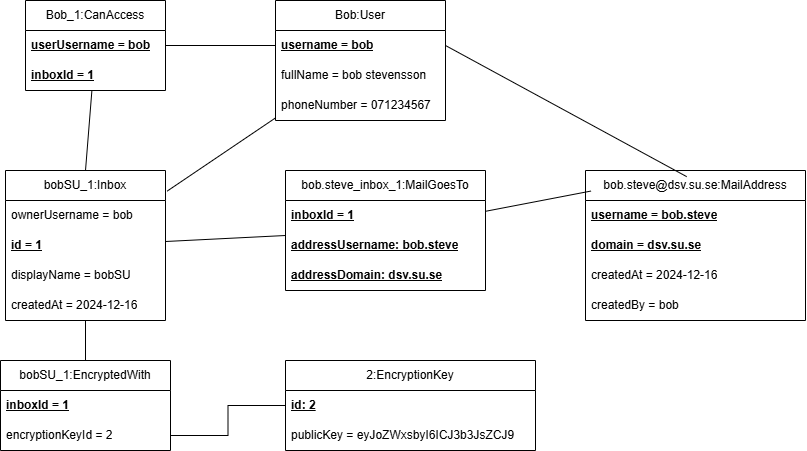
\includegraphics[width=1\textwidth]{model/instance.png}
    \caption{An instance of the database model for the email system.}
    \label{fig:instanceDatabaseModel}
\end{figure}

\section{The SQLite Implementation Tools}
\label{sqliteImplementationTools}
The following tools will be presented in this document:
\begin{itemize}
    \item DBeaver Community (see \autoref{dbeaverCommunity})
    \item SQLiteStudio (see \autoref{sqliteStudio})
    \item SQLite ERD (see \autoref{sqliteERD})
\end{itemize}

\section{DBeaver Community}
\label{dbeaverCommunity}

\subsection{Relevant Known Issues}
\label{dbeaverKnownIssues}

\subsubsection{Bad Primary Key due to auto increment}
When creating an integer column in DBeaver Community with the ``auto increment'' box checked the SQL generated will have a PK constraint created twice. This will result in an error when trying to persist the changes since a table can only have one PRIMARY KEY constraint. The following code is generated by DBeaver Community when trying to persist the changes:
\begin{lstlisting}[caption={Bad Primary Key due to auto increment in DBeaver}]
CREATE TABLE BadPK (
	Column1 INTEGER NOT NULL PRIMARY KEY AUTOINCREMENT,
	CONSTRAINT BadPK_PK PRIMARY KEY (Column1)
);
\end{lstlisting}
The solution to this is to never use the ``auto increment box'' (for a SQLite database in DBeaver) when creating a PK in the program. Unchecking the box will instead yield the following code:
\begin{lstlisting}[caption={Ok Primary Key in DBeaver if auto increment is unchecked}]
CREATE TABLE GoodPK (
	Column1 INTEGER NOT NULL,
	CONSTRAINT GoodPK_PK PRIMARY KEY (Column1)
);
\end{lstlisting}
For more information on why this is the case see \cite{dbeaver_issue_18491}.


\subsection{Common Problems}
\label{dbeaverCommonProblems}

\subsubsection{Foreign Key Constraints are not enforced}
\label{dbeaverForeignKeysNotEnforced}
DBeaver does not enforce foreign key constraints by default. This can either be enabled when creating a new database (see \autoref{dbeaverCreatingDatabase}) or by editing the database connection settings as follows:
\begin{enumerate}
    \item Right-click on the connection and choose ``Edit Connection''. (\autoref{fig:edit_connection})
    \item Go to ``Connection settings'' → ``Driver properties'' (\autoref{fig:edit_driver_properties}).
    \item Locate and change ``Foreign keys'' to ``true'' (\autoref{fig:edit_foreign_keys_enable}).
    \item Press ``OK'' and reconnect if necessary.
\end{enumerate}

\begin{figure}[!htb]
  \centering
  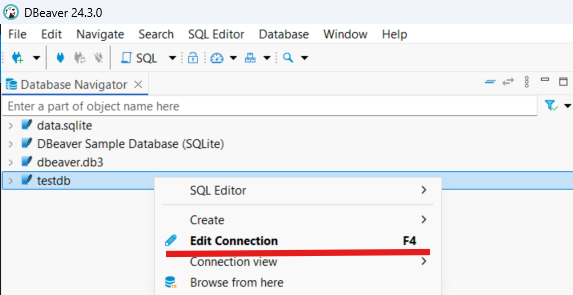
\includegraphics[width=0.7\textwidth]{dbeaver/edit_connection.png}
  \caption{Edit Connection in DBeaver.}
  \label{fig:edit_connection}
\end{figure}

\begin{figure}[!htb]
  \centering
  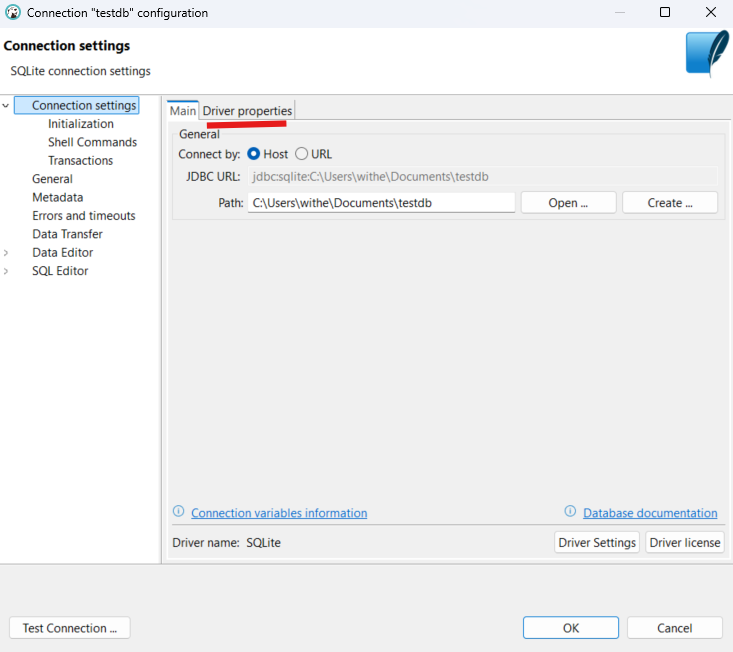
\includegraphics[width=0.7\textwidth]{dbeaver/edit_driver_properties.png}
  \caption{Driver Properties in DBeaver.}
  \label{fig:edit_driver_properties}
\end{figure}

\begin{figure}[!htb]
  \centering
  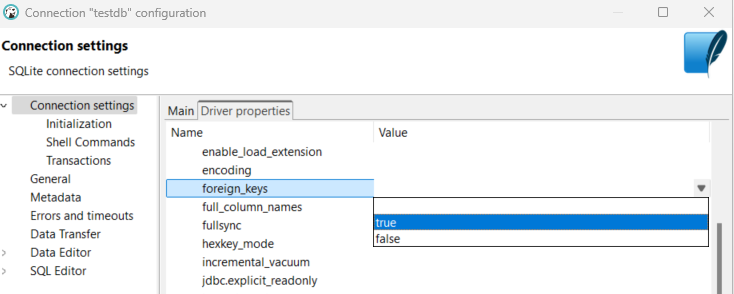
\includegraphics[width=0.7\textwidth]{dbeaver/edit_foreign_keys_enable.png}
  \caption{Enable Foreign Keys in DBeaver.}
  \label{fig:edit_foreign_keys_enable}
\end{figure}

\subsubsection{ERD Created Foreign Key Constraints}
\label{dbeaverERDCreatedForeignKeys}
The ERD tool in DBeaver Community allows you to drag tables/columns to create ``virtual keys'' which are not saved in the database itself - per the DBeaver documentation:
``Note: Virtual keys exist only in DBeaver, not in the database itself. You can define these keys even if your database does not support them.''. \cite{dbeaver_virtual_keys} So do not rely on the ERD tool to create foreign key constraints in the database itself, instead follow the steps outlined in \autoref{dbeaverForeignKeys}.

\subsubsection{Editing a Column}
\label{dbeaverEditingColumn}
It is not possible to change a columns datatype/NULL constraint/etc. after creation in DBeaver Community. The only way to change a column is to create a new column with the desired properties, copy the data (if applicable) over and subsequently delete the old column.

% \subsection{Implementation of the Database Model}
% \label{dbeaverImplementation}

\subsection{Creating Databases}
\label{dbeaverCreatingDatabase}
To create a new database with foreign key constraints enabled in DBeaver Community:
\begin{enumerate}
    \item Press ``New Database Connection'' (\autoref{fig:new_database_connection}).
    \item Choose SQLite, press ``Next''. (\autoref{fig:new_database_sqlite})
    \item Choose a file location for the database with ``Create...'' ensure to name the file with the extension ``.db3'' or ``.sqlite3'' (\autoref{fig:create_choose_file_location}).
    \item Go to ``Driver Properties'' and change ``Foreign keys'' to ``true'' (\autoref{fig:create_foreign_keys_enable}).
    \item Press ``Finish''.
\end{enumerate}

\begin{figure}[!htb]
  \centering
  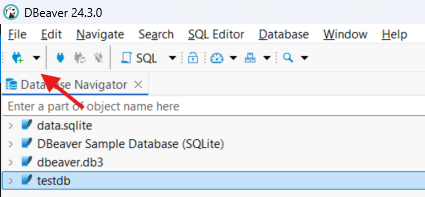
\includegraphics[width=0.7\textwidth]{dbeaver/new_database_connection.png}
  \caption{New Database Connection in DBeaver.}
  \label{fig:new_database_connection}
\end{figure}

\begin{figure}[!htb]
  \centering
  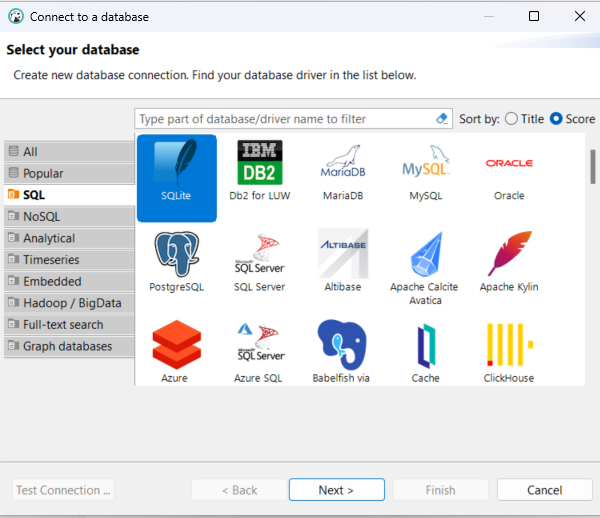
\includegraphics[width=0.7\textwidth]{dbeaver/new_database_sqlite.png}
  \caption{New SQLite Database in DBeaver.}
  \label{fig:new_database_sqlite}
\end{figure}

\begin{figure}[!htb]
  \centering
  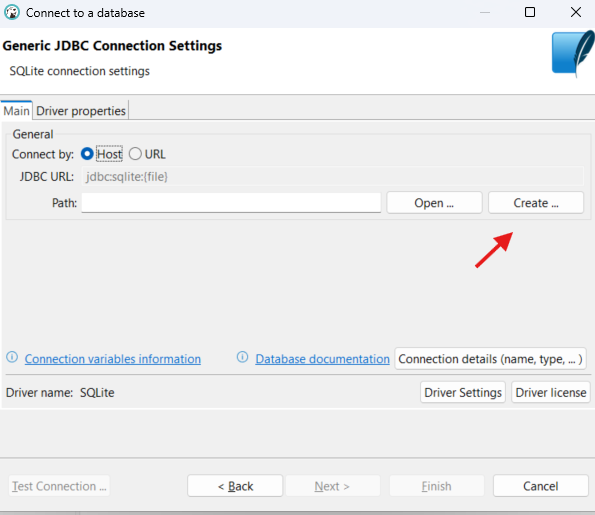
\includegraphics[width=0.7\textwidth]{dbeaver/create_choose_file_location.png}
  \caption{Choose File Location in DBeaver.}
  \label{fig:create_choose_file_location}
\end{figure}

\begin{figure}[!htb]
  \centering
  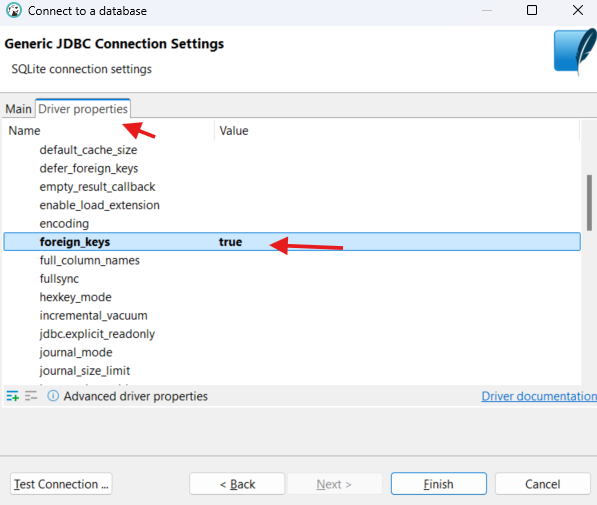
\includegraphics[width=0.7\textwidth]{dbeaver/create_foreign_keys_enable.png}
  \caption{Enable Foreign Keys in DBeaver.}
  \label{fig:create_foreign_keys_enable}
\end{figure}



\subsection{Creating Tables}
\label{dbeaverCreatingTable}
% TODO: and breifly mention MailGoesTo table
From the database model, we will be implementing the User and the MailAddress tables. The rest of the tables can be implemented similarly and is left as an exercise for the reader.

\subsubsection{User Table}
\label{dbeaverUserTable}

\begin{enumerate}
  \item \label{dbeaverCreateTable} Expand the database connection and right-click on ``Tables'' and choose ``Create New Table'' (\autoref{fig:create_new_table}).
  \item Fill out the Table Name field, navigate to the ``Columns'' tab, right click and choose ``Add Column'' (\autoref{fig:name_and_add_column}).
  \item \label{dbeaverAddColumn} Add the column for username, set the datatype to ``TEXT'', check the box for ``Not Null'' and the box for ``Unique'' in order to create a single column primary key (\autoref{fig:username_primary_key}).
  \item Repeat step \ref{dbeaverAddColumn} for the columns ``fullName'' and ``phoneNumber'' but without checking the box for ``Unique''.
  \item Save with ``Ctrl + S'' (or your operating system's equivalent) and press ``Execute''.
  \item The resulting table can be visualized using DBeaver's built in ER Diagram tool (\autoref{fig:user_er_diagram}). 
\end{enumerate}

\begin{figure}[!htb]
  \centering
  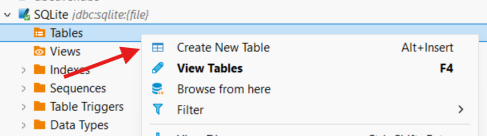
\includegraphics[width=0.7\textwidth]{dbeaver/create_new_table.png}
  \caption{Create New Table in DBeaver.}
  \label{fig:create_new_table}
\end{figure}

\begin{figure}[!htb]
  \centering
  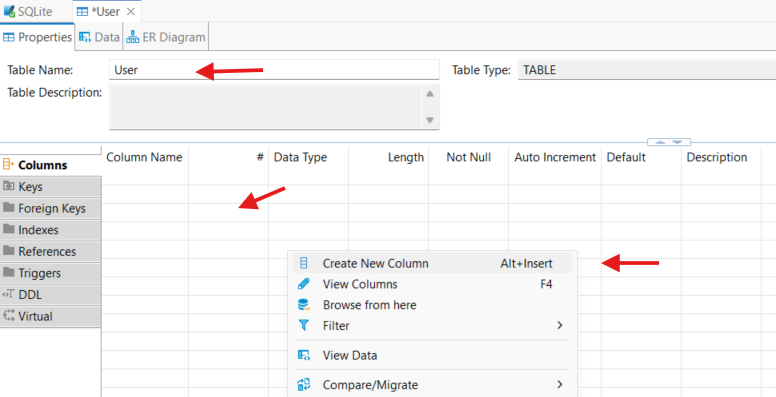
\includegraphics[width=0.7\textwidth]{dbeaver/name_and_add_column.png}
  \caption{Add Column in DBeaver.}
  \label{fig:name_and_add_column}
\end{figure}

\begin{figure}[!htb]
  \centering
  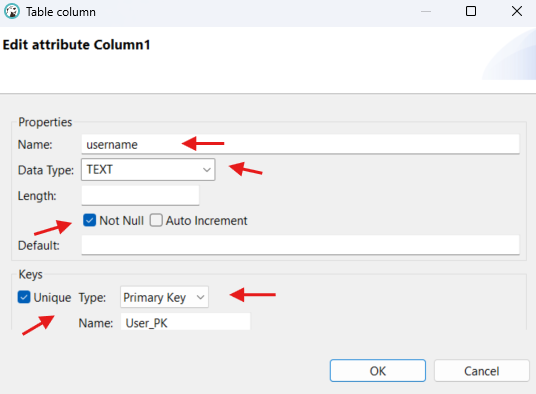
\includegraphics[width=0.7\textwidth]{dbeaver/username_primary_key.png}
  \caption{Username Primary Key in DBeaver.}
  \label{fig:username_primary_key}
\end{figure}

\begin{figure}[!htb]
  \centering
  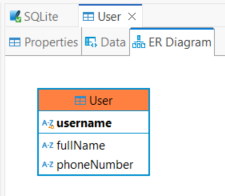
\includegraphics[width=0.7\textwidth]{dbeaver/user_er_diagram.png}
  \caption{User ER Diagram in DBeaver.}
  \label{fig:user_er_diagram}
\end{figure}


\subsubsection{MailAddress Table}
\label{dbeaverMailAddressTable}
The process for creating the MailAddress table is similar to the User table with the exception that the \textbf{primary key} is a composite key. The PK for the table consists of the columns ``username'' and ``domain''. Steps for creating columns are the same as for \ref{dbeaverUserTable}, creating the composite key is done as follows:
\begin{enumerate}
  \item Navigate to the ``Keys'' tab (\autoref{fig:table_keys_navigate}).
  \item Right click, choose ``Create New Key''
  \item Set the type to ``Primary Key'' and tick the columns ``username'' and ``domain'' to the key (\autoref{fig:mail_address_primary_key}).
  \item Press ``OK'' and save the table.
  \item The resulting table can be visualized using DBeaver's built in ER Diagram tool. (\autoref{fig:mail_address_er_diagram})
\end{enumerate}

\begin{figure}[!htb]
  \centering
  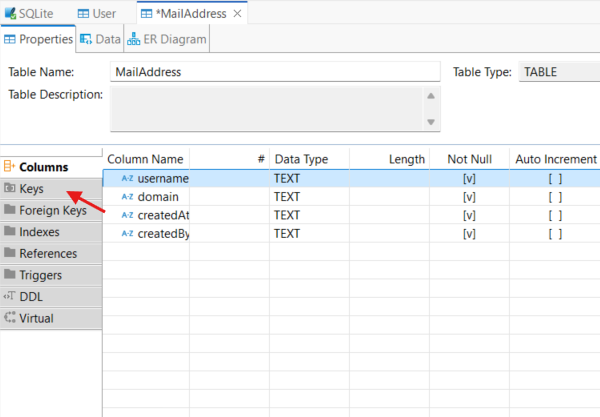
\includegraphics[width=0.7\textwidth]{dbeaver/table_keys_navigate.png}
  \caption{Navigate to Keys in DBeaver.}
  \label{fig:table_keys_navigate}
\end{figure}

\begin{figure}[!htb]
  \centering
  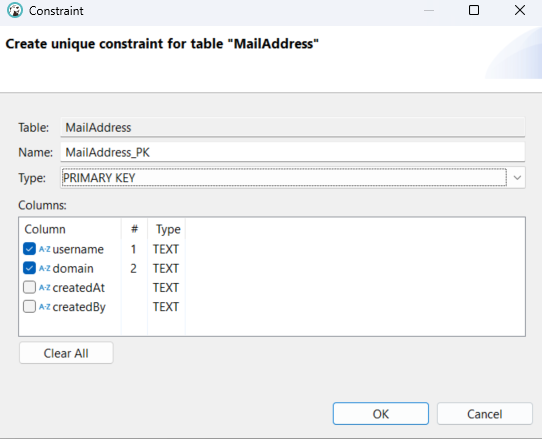
\includegraphics[width=0.7\textwidth]{dbeaver/mail_address_primary_key.png}
  \caption{MailAddress Primary Key in DBeaver.}
  \label{fig:mail_address_primary_key}
\end{figure}

\begin{figure}[!htb]
  \centering
  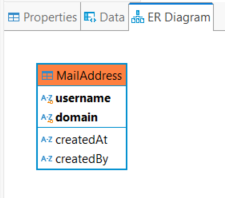
\includegraphics[width=0.7\textwidth]{dbeaver/mail_address_er_diagram.png}
  \caption{MailAddress ER Diagram in DBeaver.}
  \label{fig:mail_address_er_diagram}
\end{figure}

\subsubsection{MailGoesTo Table}
\label{dbeaverMailGoesToTable}
The process of creating the MailGoesTo table is almost identical to the \autoref{dbeaverMailAddressTable} with the exception that all columns are part of the primary key. The resulting table can be visualized with DBeaver as \autoref{fig:mail_goes_to_er_diagram}.

\begin{figure}[!htb]
  \centering
  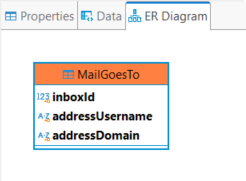
\includegraphics[width=0.7\textwidth]{dbeaver/mail_goes_to_er_diagram.png}
  \caption{MailGoesTo ER Diagram in DBeaver.}
  \label{fig:mail_goes_to_er_diagram}
\end{figure}

\subsection{Alternative Keys}
\label{dbeaverAlternativeKeys}
To create an alternative key (unique index) in DBeaver this can be exemplified on User by declaring that the columns ``fullName'' and ``phoneNumber'' should be unique together. This can be done as follows:

\begin{enumerate}
  \item Navigate to the ``Indexes'' tab in the User table (\autoref{fig:user_index_tab}).
  \item Right-click and choose ``Create New Index''.
  \item Select the columns ``fullName'' and ``phoneNumber'', tick the box for ``Unique'' and press ``OK''. (\autoref{fig:user_index_create})
\end{enumerate}

\begin{figure}[!htb]
  \centering
  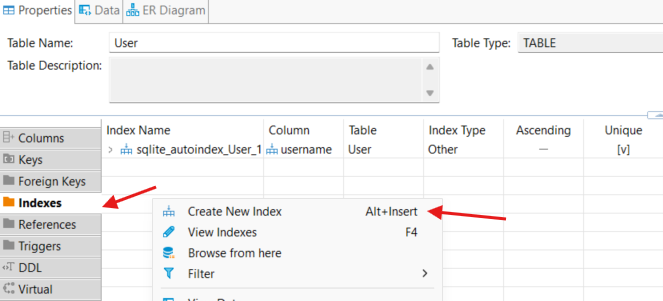
\includegraphics[width=0.7\textwidth]{dbeaver/user_index_tab.png}
  \caption{Navigate to Indexes in DBeaver.}
  \label{fig:user_index_tab}
\end{figure}

\begin{figure}[!htb]
  \centering
  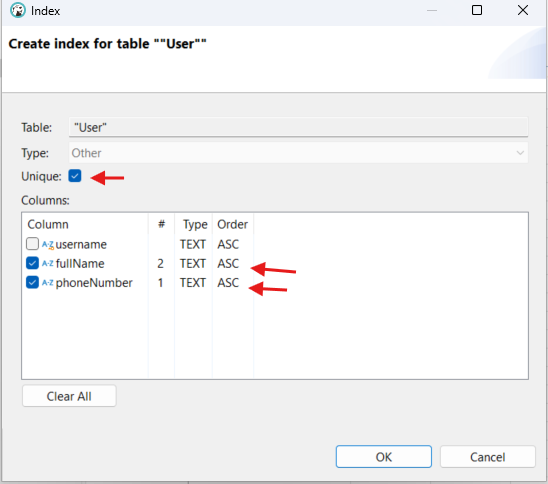
\includegraphics[width=0.7\textwidth]{dbeaver/user_index_create.png}
  \caption{Create Unique Index in DBeaver.}
  \label{fig:user_index_create}
\end{figure}


\subsection{Foreign Keys}
\label{dbeaverForeignKeys}
Creating foreign keys in DBeaver will be exemplified on the relationships between MailAddress.(createdBy) → User.(username) and MailGoesTo.(username, domain) → MailAddress.(username, domain).

\subsubsection{MailAddress → User}
\label{dbeaverUserMailAddressRelationship}
A single column foreign key relationship between User.(username) and MailAddress.(createdBy), can be created as follows:

\begin{enumerate}
  \item Navigate to the ``Foreign Keys'' tab of the MailAddress table.
  \item Right-click and choose ``Create New Foreign Key''. (\autoref{fig:navigate_create_foreign_key_tab}).
  \item Set the destination / ``reference'' table to User, the ``from'' column to createdBy and the reference column to username. (\autoref{fig:create_foreign_key_mail_address_user}).
  \item Set ``ON DELETE'' and ``ON UPDATE'' to appropriate values.
  \item Press ``OK'' and save the table.
\end{enumerate}

\begin{figure}[!htb]
  \centering
  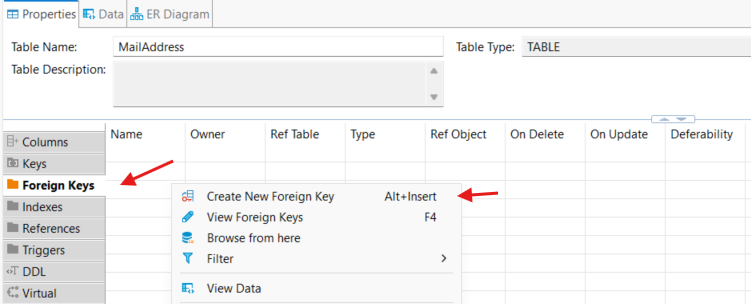
\includegraphics[width=0.7\textwidth]{dbeaver/navigate_create_foreign_key_tab.png}
  \caption{Navigate to Create Foreign Key in DBeaver.}
  \label{fig:navigate_create_foreign_key_tab}
\end{figure}

\begin{figure}[!htb]
  \centering
  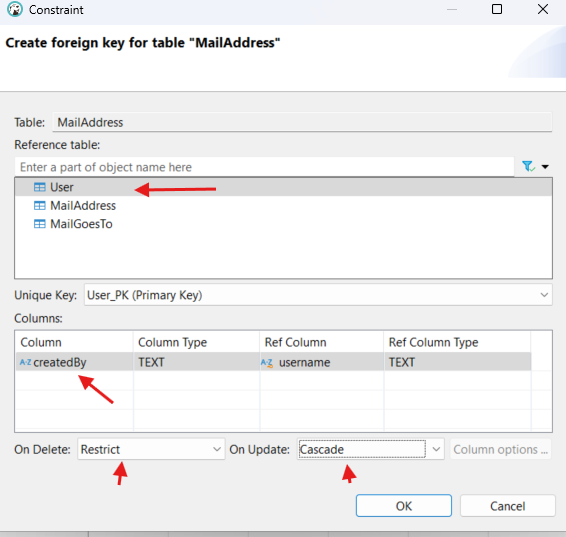
\includegraphics[width=0.7\textwidth]{dbeaver/create_foreign_key_mail_address_user.png}
  \caption{Create Foreign Key MailAddress → User in DBeaver.}
  \label{fig:create_foreign_key_mail_address_user}
\end{figure}



\subsubsection{MailGoesTo → MailAddress}
\label{dbeaverMailGoesToMailAddressRelationship}
C composite foreign key relationship between MailGoesTo.(addressUsername, addressDomain) and MailAddress.(username, domain), can be created as follows:

\begin{enumerate}
  \item Navigate to the ``Foreign Keys'' tab of the MailGoesTo table.
  \item Right-click and choose ``Create New Foreign Key''. (\autoref{fig:navigate_create_foreign_key_tab}).
  \item Set the destination / ``reference'' table to MailAddress, the ``from'' columns to username and domain and the reference columns to username and domain. (\autoref{fig:create_foreign_key_mail_goes_to_mail_address}).
  \item Set ``ON DELETE'' and ``ON UPDATE'' to appropriate values.
  \item Press ``OK'' and save the table.
\end{enumerate}

\begin{figure}[!htb]
  \centering
  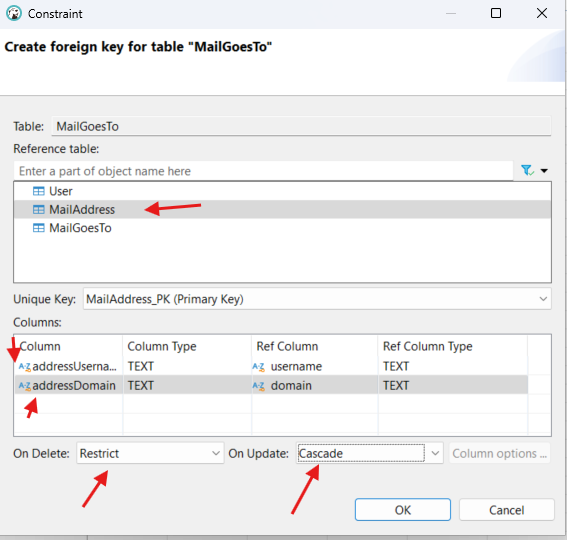
\includegraphics[width=0.7\textwidth]{dbeaver/create_foreign_key_mail_goes_to_mail_address.png}
  \caption{Create Foreign Key MailGoesTo → MailAddress in DBeaver.}
  \label{fig:create_foreign_key_mail_goes_to_mail_address}
\end{figure}


\subsection{Inserting Data}
\label{dbeaverInsertingData}

We will now insert data into the User and MailAddress tables. The data to be inserted can be seen in \autoref{fig:instanceDatabaseModel}. The process for inserting data is the same for all tables and can be exemplified on the User table as follows:

\begin{enumerate}
  \item Navigate to the ``Data'' tab of the User table.
  \item Right-click, choose ``Edit'' and then ``Add Row''. (\autoref{fig:insert_data_user})
  \item Fill out the data for the columns. (\autoref{fig:insert_data_user_populated})
  \item Press ``Ctrl + S'' (or your operating system's equivalent) to save the data.
\end{enumerate}

For foreign key relationships, referencial integrity will be enforced assuming the foreign key constraints are enabled (see \autoref{dbeaverCreatingDatabase} or \autoref{dbeaverForeignKeysNotEnforced}).

\begin{figure}[!htb]
  \centering
  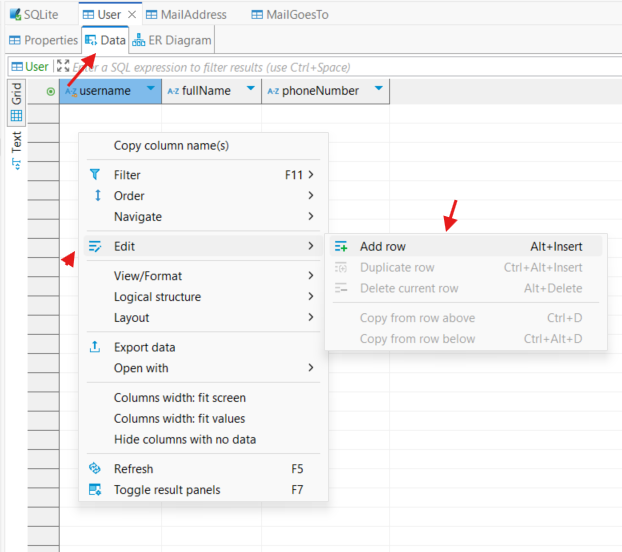
\includegraphics[width=0.7\textwidth]{dbeaver/insert_data_user.png}
  \caption{Insert Data into User in DBeaver.}
  \label{fig:insert_data_user}
\end{figure}

\begin{figure}[!htb]
  \centering
  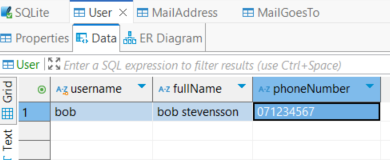
\includegraphics[width=0.7\textwidth]{dbeaver/insert_data_user_populated.png}
  \caption{Bob User Populated in DBeaver.}
  \label{fig:insert_data_user_populated}
\end{figure}


\subsection{Querying Data}
\label{dbeaverQueryingData}

Queries can be written and executed using the views section in DBeaver. The following query will return all columns from the User table where the users full name is ``bob stevensson''.

\begin{lstlisting}[caption={Querying Data in DBeaver}]
SELECT
  *
FROM
  User,
  MailAddress
WHERE
  User.username = MailAddress.createdBy
  AND User.fullName = 'bob stevensson';
\end{lstlisting}

And the process for doing this in DBeaver is as follows:
\begin{enumerate}
  \item Right-click on ``Views'' and choose ``Create New View''. (\autoref{fig:create_view})
  \item Give the view a name and navgiate to definition and write the query. (\autoref{fig:view_bob_emails_define})
  \item Press ``Ctrl + S'' (or your operating system's equivalent) to save the view.
  \item Navigate to the ``Data'' tab of the view to see the result. (\autoref{fig:view_bob_emails_result})
\end{enumerate}


\begin{figure}[!htb]
  \centering
  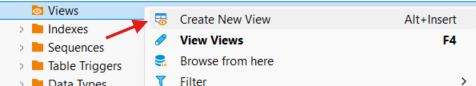
\includegraphics[width=0.7\textwidth]{dbeaver/create_view.png}
  \caption{Create View in DBeaver.}
  \label{fig:create_view}
\end{figure}

\begin{figure}[!htb]
  \centering
  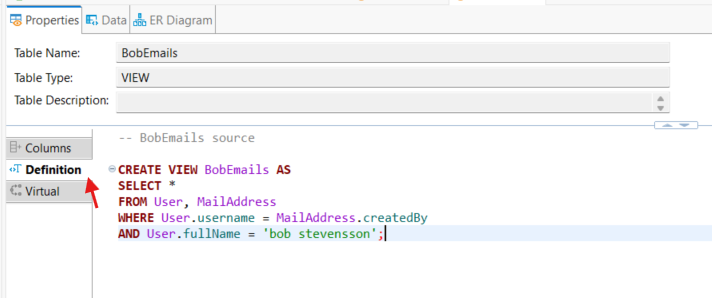
\includegraphics[width=0.7\textwidth]{dbeaver/view_bob_emails_define.png}
  \caption{Define View in DBeaver.}
  \label{fig:view_bob_emails_define}
\end{figure}

\begin{figure}[!htb]
  \centering
  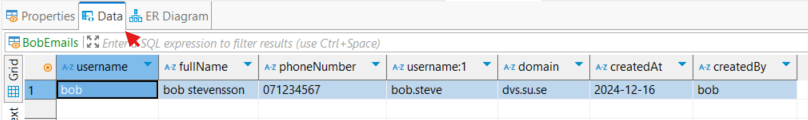
\includegraphics[width=0.8\textwidth]{dbeaver/view_bob_emails_result.png}
  \caption{Result of View in DBeaver.}
  \label{fig:view_bob_emails_result}
\end{figure}

\section{SQLiteStudio}
\label{sqliteStudio}

\subsection{Relevant Known Issues}
\label{sqliteStudioKnownIssues}
Nothing to note at this time!

\subsection{Common Problems}
\label{sqliteStudioCommonProblems}

\subsubsection{Table Not Saved}
\label{sqliteStudioTableNotSaved}
When creating a table in SQLiteStudio the table is not saved until the changes are persisted and progress might be discarded if another table / tab is accessed before saving. This can be mitigated by saving the table directly after creation via ``Ctrl + S'' (or your operating system's equivalent).

\subsubsection{No Primary Key}
\label{sqliteStudioNoPrimaryKey}
While creating a table in SQLiteStudio it is possible to create a table without explcitly defining a primary key (this is due to how SQLite handles primary keys). This is not an error but all tables should have an explicit primary key defined.


% warning wrong datatype on FN (this is a logical error!)
\subsubsection{Wrong Datatype for Foreign Key}
\label{sqliteStudioWrongDatatypeForeignKey}
When creating a foreign key in SQLiteStudio where the datatype of the foreign key column is not the same as the column in the referenced table the program will display a warning. This is usually a logical error and should not be ignored and the datatype in the from or to column should be changed to match. The warning can be seen in \autoref{fig:badfndatatype}.


\begin{figure}[!htb]
  \centering
  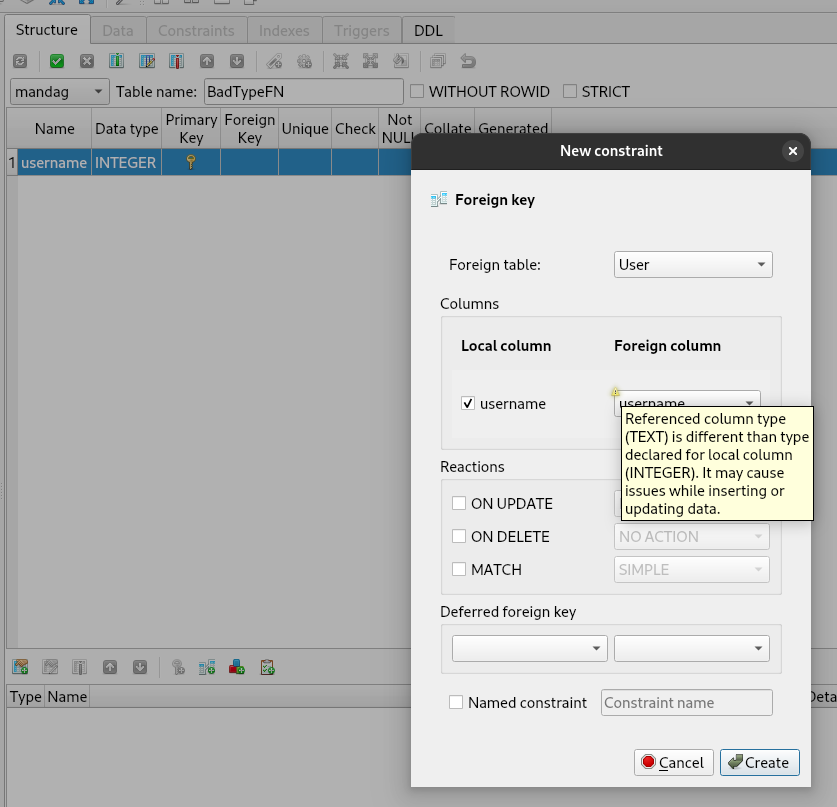
\includegraphics[width=0.8\textwidth]{sqlitestudio/badfndatatype.png}
  \caption{Wrong Datatype for Foreign Key Column in SQLiteStudio.}
  \label{fig:badfndatatype}
\end{figure}




% \subsection{Implementation of the Database Model}
% \label{sqliteStudioImplementation}

\subsection{Creating a Database}
\label{sqliteStudioCreatingDatabase}

\subsection{Creating a Table}
\label{sqliteStudioCreatingTable}

\subsubsection{User Table}
\label{sqliteStudioUserTable}

\subsubsection{MailAddress Table}
\label{sqliteStudioMailAddressTable}

\subsubsection{MailGoesTo Table}
\label{sqliteStudioMailGoesToTable}

\subsection{Alternative Keys}
\label{sqliteStudioAlternativeKeys}
% composite must be shown

\subsection{Foreign Keys}
\label{sqliteStudioForeignKeys}

\subsection{Inserting Data}
\label{sqliteStudioInsertingData}

\subsection{Querying Data}
\label{sqliteStudioQueryingData}
% queries should be saved as Views

\section{SQLite ERD}
\label{sqliteERD}
SQLite ERD is an application that can be used to create Entity Relationship Diagrams (ERDs) for SQLite databases. The application is platform independent and is used within a web browser. The application can be found at \url{https://sqlite-erd.e-su.se/}. For the interested reader the source code can be found at \url{https://github.com/Edwinexd/sqlite-erd}.
The application supports most common file formats for SQLite databases, only requiring that the file is a SQLite database of version 3.

% TODO: include figure generated from sqlite-erd

\section{Final Words}
\label{finalWords}
If you have any questions or issues with the tools presented in this document or the document itself please create an issue at \url{https://github.com/Edwinexd/db-sqlite-tools/issues}.


\pagebreak
\bibliographystyle{IEEEtran}
\bibliography{bibtex}
\bibdata{bibtex}

\end{sloppypar}
\end{document}
